\documentclass{acm_proc_article-sp}

\usepackage[T1]{fontenc}
\usepackage{polyglossia}
\setdefaultlanguage{english}
\usepackage{csquotes}

\usepackage{fontspec}
\usepackage{xltxtra}
\usepackage{libertine}

\usepackage[usenames, dvipsnames]{xcolor}
\graphicspath{{./img/}}

\usepackage[backend=biber, style=alphabetic]{biblatex}
\bibliography{literatur.bib}

\usepackage{subcaption}

\usepackage[%
unicode=true,%
colorlinks=true,%
linkcolor=black,%
urlcolor=MidnightBlue,%
citecolor=black,%
filecolor=black%
]
{hyperref}


\newcommand{\todo}[1]{\textcolor{Red}{#1}}
\newcommand{\sebastian}[1]{\textcolor{Green}{#1}}
\newcommand{\stefan}[1]{\textcolor{BurntOrange}{#1}}

\begin{document}

\title{
Interactive Simulation WS 15/16\\ %
Project Proposal
}
\subtitle{EYES - Exchange Your Vision Simulator}
\numberofauthors{2}
\author{
% 1st. author
\alignauthor
Sebastian Lemp\\
%       \affaddr{Street, House}\\
%       \affaddr{PLZ City}\\
%       \affaddr{Country}\\
%       \email{sebastian.lemp@student.uni-augsburg.de}
% 2nd. author
\alignauthor
Stefan Büttner\\
%       \affaddr{Street, House}\\
%       \affaddr{PLZ City}\\
%       \affaddr{Country}\\
%       \email{stefan.buettner@student.uni-augsburg.de}
}
%\additionalauthors{Additional Authors}

% The date is actually not used in the acm template
\date{University of Augsburg, \today}

% Not neede for our purposes
%\terms{Terms}
%\keywords{Keyword 1, Keyword 2}
%% A category with the (minimum) three required fields
%\category{H.4}{Information Systems Applications}{Miscellaneous}
%%A category including the fourth, optional field follows...
%\category{D.2.8}{Software Engineering}{Metrics}[complexity measures, performance measures]

%% For the ACM ToG format
%\acmformat{ACMFormat}
%\acmVolume{Vol.}
%\acmNumber{Nr.}
%\acmYear{YYYY}
%\acmMonth{MM}
%\acmArticleNum{XXX}
%\doi{DOI}


\maketitle
%\begin{abstract}
%\end{abstract}

\section{Introduction/Motivation}
\begin{itemize}
  \item Give people the opportunity to experience other perception systems
  than the human eye ⇒ understanding why moths are caught by light, why
  flies fly in your eye while bicycling, why flies fly against glass...

\end{itemize}

\sebastian{willst du die moths reinbringen wenn wir die evenutell nicht machen?
Sondern lieber nen Beispiel mit Bienen}\\
\stefan{Weiss noch net. Wenn wir die net machen, dann net. Hab bisher lediglich
die meisten Gedanken, die mir durch den Kopf gegangen sind niedergeschrieben.}



\section{Concept}
\begin{itemize}
\item At least 2 other visual systems to choose from
\item One or more tasks to solve using those available systems.
  \begin{itemize}
    \item Find a flower or some sweets (Bee/Wasp)
    \item Find something and return to the colony as fast as possible (Ant)
    \item Go as far as possible in the night without dying (moth)
    \item Find an exit to the room/café/drinking glass (caught by some human)/...
    \item Cross the highway
  \end{itemize}
\item Model the visual systems as realistically as possible.
\item Use oculus rift / Google Cardboard to address each eye individually
→ different modes:
  \begin{itemize}
  \item Both human eyes see the same images to have a flat, monitor like view
  \item For binocular systems: One-to-one mapping of the eyes
        For multiocular systems: Map them somehow to the two human eyes
  \end{itemize}
\end{itemize}

\sebastian{Ich würde glaub ich das mit oculus rift / cardboard rausnehmen,
Will es zwar auch umbedingt machen aber weiß nicht ob wir den fokus auf ne pc
version lenken sollten. Aufgrund der eventuellen komplexität}\\
\stefan{Nee, ich würd's schon reinschreiben. Weil ich finde das wäre schon ein
zentraler Punkt des Projekts. Klar machen wir uns dadurch auch etwas Druck,
aber muss. Aber dafür können wir ja vllt. bis Mo kurz schauen, ob ne Oculus Rift
Integration eher schwer oder eher einfach ist und es danach entscheiden.}



\begin{figure}
  \centering
  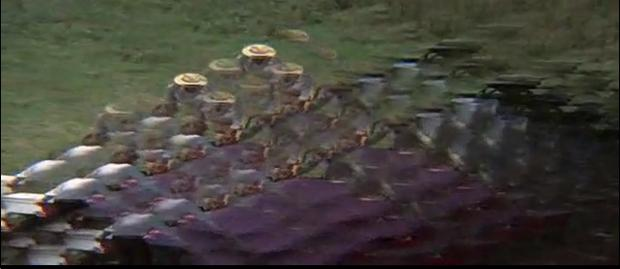
\includegraphics[width=0.4\textwidth]{bee-vision.jpg}
  \caption{Qualitative retina image captured by an apposition eye.}
  \label{appositeeye}
\end{figure}

\begin{centering}
\begin{figure}
  \begin{subfigure}[t]{0.1345\textwidth}
    \centering
    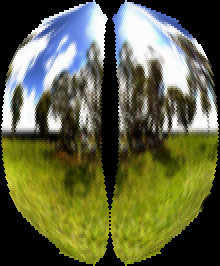
\includegraphics[width=\textwidth]{beeview.png}
    \caption{Rendering of an environment as seen by a bee.}
    \label{beeview}
  \end{subfigure}
  ~
  \begin{subfigure}[t]{0.3255\textwidth}
    \centering
    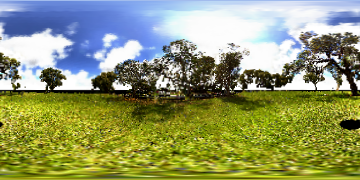
\includegraphics[width=\textwidth]{beeview-panorama.png}
    \caption{Panorama rendering of the scene.}
    \label{beeviewpanorama}
  \end{subfigure}
  \caption{Renderings generated by InsectVision \cite{insectvision}.}
\end{figure}
\end{centering}

\subsection{User Experience}

\section{Project Requirements}
\todo{Cite this whole shit}\\
The pinhole camera model used in most computer graphics software to mimic
the human visual perception is a rather crude approximation to the real world.
We do not recognize this most of the time, because we are used to it. In other
words, our brains do a lot of preprocessing.
One example is the \emph{blind spot} where the optic nerve exits the eye.
In this area there are no photoreceptor cells and thus no visual information is
available. Yet, we don't notice this in everyday life since the brain merges
the information of the left and the right eye and compensates this lack of
information. Other effects are optical distortion or color sensitivity which
is not uniform over the retina.
Nevertheless, using this pinhole model yields better results on computer screen
or a virtual reality device, actually the ones we expect. In contrast,
displaying the image captured by the retina of a human eye would not yield
satisfying results (\todo{describe them?}).
Yet, the only thing we can do about other animals visual systems is reconstruct
this image as closely as possible and invent mappings of those images to our
eyes which we believe come close to the actual perception.
This is especially evident when looking at species with more than two eyes.

The same goes for the perceived range of the visual spectrum. If the perceived
range exceeds the spectrum visible to humans, a remapping is required.

\todo{Give the user/player the freedom to design or influence this retina image
to human-eye mapping? E.g. the spectral mapping could be influenced quite easily
because it's from ℝ to ℝ.}

The eyes of honey bees are already well studied. There are measurements
of the ommatidial density on the eye ellipsoid as well as the spectral
sensitivity of the ommatidia. Therefor an accurate model can be derived.
Scientist of the German Aerospace Center in cooperation with the Australian
National University, for example, implemented a renderer
which renders a panorama image from the view of a bee \cite{insectvision}
in order to study the way bees navigate almost without any depth perception and
low image resolution.
Another project at the University of Sussex realized a VR-game where the
player is supposed to find as many flowers as possible in a given time
period \cite{beepilot}.
Yet, both of these project did not take the spectral sensitivity of the bees
into account. Therefor this project's novum is to represent the bee's spectral
perception in some way.

Unlike humans, bee's are less sensitive to red but more sensitive to green and
ultra violet wavelengths \todo{cite}. They are even capable of recognizing the
polarization of the light because the photoreceptive cells in each ommatidium
respond to different polarizations differently.
Altough all of this is really interesting, we don't know yet to what extent those
aspects are going to be realized. This is due to our current lack of technical
knowledge about Unity3D and the principal difficulty how to display these
effects.

\begin{description}
  \item[Science]
% - Optical apparatus and movement of different species, e.g.
%     Flies, Spiders, Wasps, Bees, Bats (sonic perception?),
%     fish (deep sea?), birds, simple cellular organisms
% - Mapping of the perceived spectra of the different species to the human
%   perceivable spectrum (papers on this topic)
% - How is polarized light perceived?
% - Mapping of the layout of one system to the human visual system
% See \cite{insectvision}
  \sebastian{Sollten wir dies nicht genauer beschreiben? Also genau welche wir
  vorhaben zu machen? ( Bienen/Fliegen?)}\\
  \stefan{Jap, aber das ist immernoch die Ideensammlung von So einfach
  reinkopiert.}

\item[Different eye types]
% \begin{itemize}
%   \item Simple eyes
%   \begin{itemize}
%     \item Pit
%     \item Spherical lensed
%     \item Multiple lenses
%     \item Refractive cornea
%     \item Reflector
%   \end{itemize}
%   \item Compound eyes
%   \begin{itemize}
%     \item Apposition
%     \item Superposition
%     \item Parabolic superposition
%   \end{itemize}
% \end{itemize}
\sebastian{Auch evenutell genauer? Bezüglich was wir machen.}\\
\stefan{Ist nur ne Übersicht um bissel Info zu haben und dass es nach mehr
aussieht :P}

\item[Gamification]
- Search targets with different eyes. Different species have different
  \"standard\" activities.
  Implement one/two/... which can be solved with any vision system.
  I.e. All n vision systems can be chosen in all m species specific activities,
  or to put it differently: Equip character with another vision system.
  E.g. Ant foraging: search food and return to base as fast as possible.
- Possibility to create your own vision system by configuring n eyes(cameras)
  and attach them to the model (ant, spider, whatever) and choose a layout
  for the 2D-screen / oculus.
  /sebastian{weis nicht ob ich das auch rausnehmen würde}
  This lets the user test and develop better, task specific visual systems.
  Of course: save/load
- Species-task specific companions/enemies which need to be simulated

\item[Complexity]
- In combination with the oculus rift: visual complexity in
  processing/perceiving the environment.
- learning about the visual systems of other species
- Dunno about model complexity, yet.

\sebastian{Wie oben würde ich mich glaube nicht so auf OR fixieren oder
zumindestens es als untersten Punkt nennen.}\\
\stefan{\href{https://www.youtube.com/watch?v=F54ME85o_aQ}
{Aber ich mag doch die Oculus...}}


\item[Aesthetics]
\end{description}

\sebastian{Bezüglich Aesthetics: Da würde ich einfach die Basic sachen trozdem
nochmal reinschreiben: 3D, firstperson, etc...}\\
\stefan{Okay, mach ;)}


\section{Timeline}

Todos:
\begin{itemize}
  \item Research
  \begin{itemize}
    \item How to model the eyes of a bee?
    \item How to implement custom camera projections in Unity?
    \item How to realize spectral rendering?
    \item What other visual systems are well known to be implemented? → Fiddler Crab
    \item How to model the eyes of this othe species?
    \item How to interface with the oculus ritf?
    \item Obtain model for infrared/ultraviolet light transport in real life
          scenarios along realistic values for materials and emmiters (sun/sky/lamps/...)
  \end{itemize}
  \item Implementation
  \begin{itemize}
    \item Implement bee sight
    \item Implement other sight
    \item Create scenario/level 1
    \item Create another scenario
    \item Create menu
    \item Based on level: Implement threats
    \item Integrate oculus rift
  \end{itemize}
  \item Testing
\end{itemize}

\begin{center}
  \begin{tabular}{|l|p{6.5cm}|}
    \hline
    Oct. '15 & uiae \\ \hline
    Nov. '15 & xvlc \\ \hline
    Dec. '15 & asdf \\ \hline
    Jan. '15 & qwer \\ \hline
    Feb. '15 & foo \\
    \hline
  \end{tabular}
\end{center}

\printbibliography

\balancecolumns

\end{document}
